% https://tex.stackexchange.com/a/483817/173708
\documentclass[tikz]{standalone}
\usetikzlibrary{decorations.pathreplacing,positioning, arrows.meta}
\begin{document}
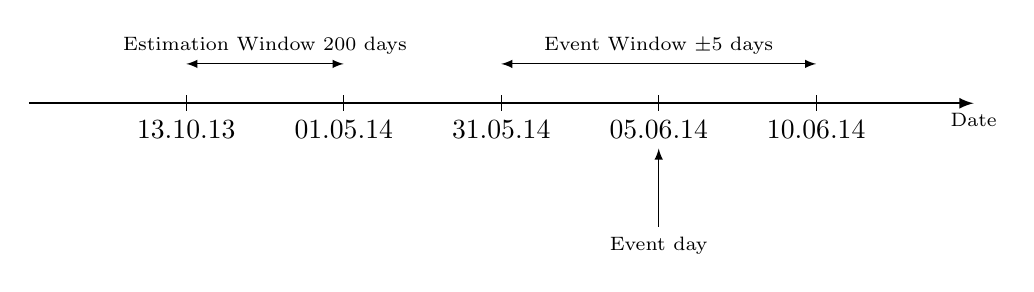
\begin{tikzpicture}[x=2cm,>=latex]
	\draw[thick,->] (0,0) -- (6,0) node[below,font=\scriptsize] {Date};
	\draw (1,.1)--(1,-.1) node[below] {13.10.13};
	\draw (2,.1)--(2,-.1) node[below] {01.05.14};
	\draw (3,.1)--(3,-.1) node[below] {31.05.14};
	\draw (4,.1)--(4,-.1) node[below] (x) {05.06.14};
	\draw (5,.1)--(5,-.1) node[below] {10.06.14};
	
	\draw[<->] (1,.5)--(2,.5) node[midway,above,font=\scriptsize] {Estimation Window 200 days};
	\draw[<->] (3,.5)--(5,.5) node[midway,above,font=\scriptsize] {Event Window $\pm5$ days};
	\draw[<-] (x.south) --++ (0,-1) node[below,font=\scriptsize] {Event day};
\end{tikzpicture}
\end{document}